% D2 - Pure Kappa Layered Architecture. The report's centerpiece.
%
% Labelled in the coursework's vocabulary: Ingestion, Stream Processing, Storage,
% Serving, Orchestration and Observability.
% In pure Kappa, there is NO speed/batch layer split: ONE unified stream processing engine
% evaluates NEWS2 and lab multipliers for both real-time triage and historical replay.
% Every technology is named; the legend fixes the colour convention.
\documentclass[border=6pt,varwidth=false]{standalone}
% Shared styling for every Kappa report diagram.
%
% Colour convention across diagrams:
%   BLUE       stream path     - unified streaming engine and message broker
%   GREEN      storage layer   - query-first Cassandra tables and master log
%   ORANGE     serving layer   - low-latency FastAPI endpoints
%   RED        clinical alerts - acute deterioration notifications
%   GREY       infrastructure  - orchestrators, metrics and supporting daemons
%
% TikZ rather than raster graphics ensures vector resolution and matching typography.

\usepackage{amsmath}
\usepackage{tikz}
\usepackage{xcolor}
\usetikzlibrary{positioning,arrows.meta,fit,backgrounds,calc,shapes.geometric,decorations.pathreplacing}

\definecolor{streamblue}{HTML}{0078D7}
\definecolor{streambg}{HTML}{E6F2FB}
\definecolor{storegreen}{HTML}{2E7D4A}
\definecolor{storebg}{HTML}{E4F3E8}
\definecolor{servorange}{HTML}{C2660A}
\definecolor{servbg}{HTML}{FCEDDD}
\definecolor{alertred}{HTML}{D83B01}
\definecolor{alertbg}{HTML}{FDE7E9}
\definecolor{infragrey}{HTML}{5A6672}
\definecolor{infrabg}{HTML}{ECEFF1}
\definecolor{edgegrey}{HTML}{444C54}

\tikzset{
  box/.style={
    draw, rounded corners=2pt, align=center, inner sep=5pt,
    font=\scriptsize, minimum height=8mm, line width=0.5pt,
  },
  stream/.style={box, draw=streamblue, fill=streambg, text=black},
  store/.style ={box, draw=storegreen, fill=storebg,  text=black},
  serv/.style  ={box, draw=servorange, fill=servbg,   text=black},
  alert/.style ={box, draw=alertred,   fill=alertbg,  text=black},
  infra/.style ={box, draw=infragrey,  fill=infrabg,  text=black},
  ext/.style   ={box, draw=edgegrey,   fill=white, dashed, text=black},
  cqlbox/.style={
    draw=storegreen, fill=white, rounded corners=1.5pt,
    align=left, inner sep=3pt, font=\tiny, line width=0.4pt
  },
  flow/.style  ={-{Stealth[length=4pt]}, draw=edgegrey, line width=0.5pt},
  streamflow/.style={flow, draw=streamblue, line width=0.7pt},
  alertflow/.style={flow, draw=alertred, line width=0.7pt},
  lbl/.style   ={font=\tiny\itshape, text=edgegrey, fill=white, inner sep=1.5pt},
  zone/.style  ={draw=edgegrey, dashed, rounded corners=3pt, line width=0.4pt, inner sep=7pt},
  ztitle/.style={font=\scriptsize\bfseries, text=edgegrey, fill=white, inner xsep=3pt, inner ysep=1pt},
}

\begin{document}
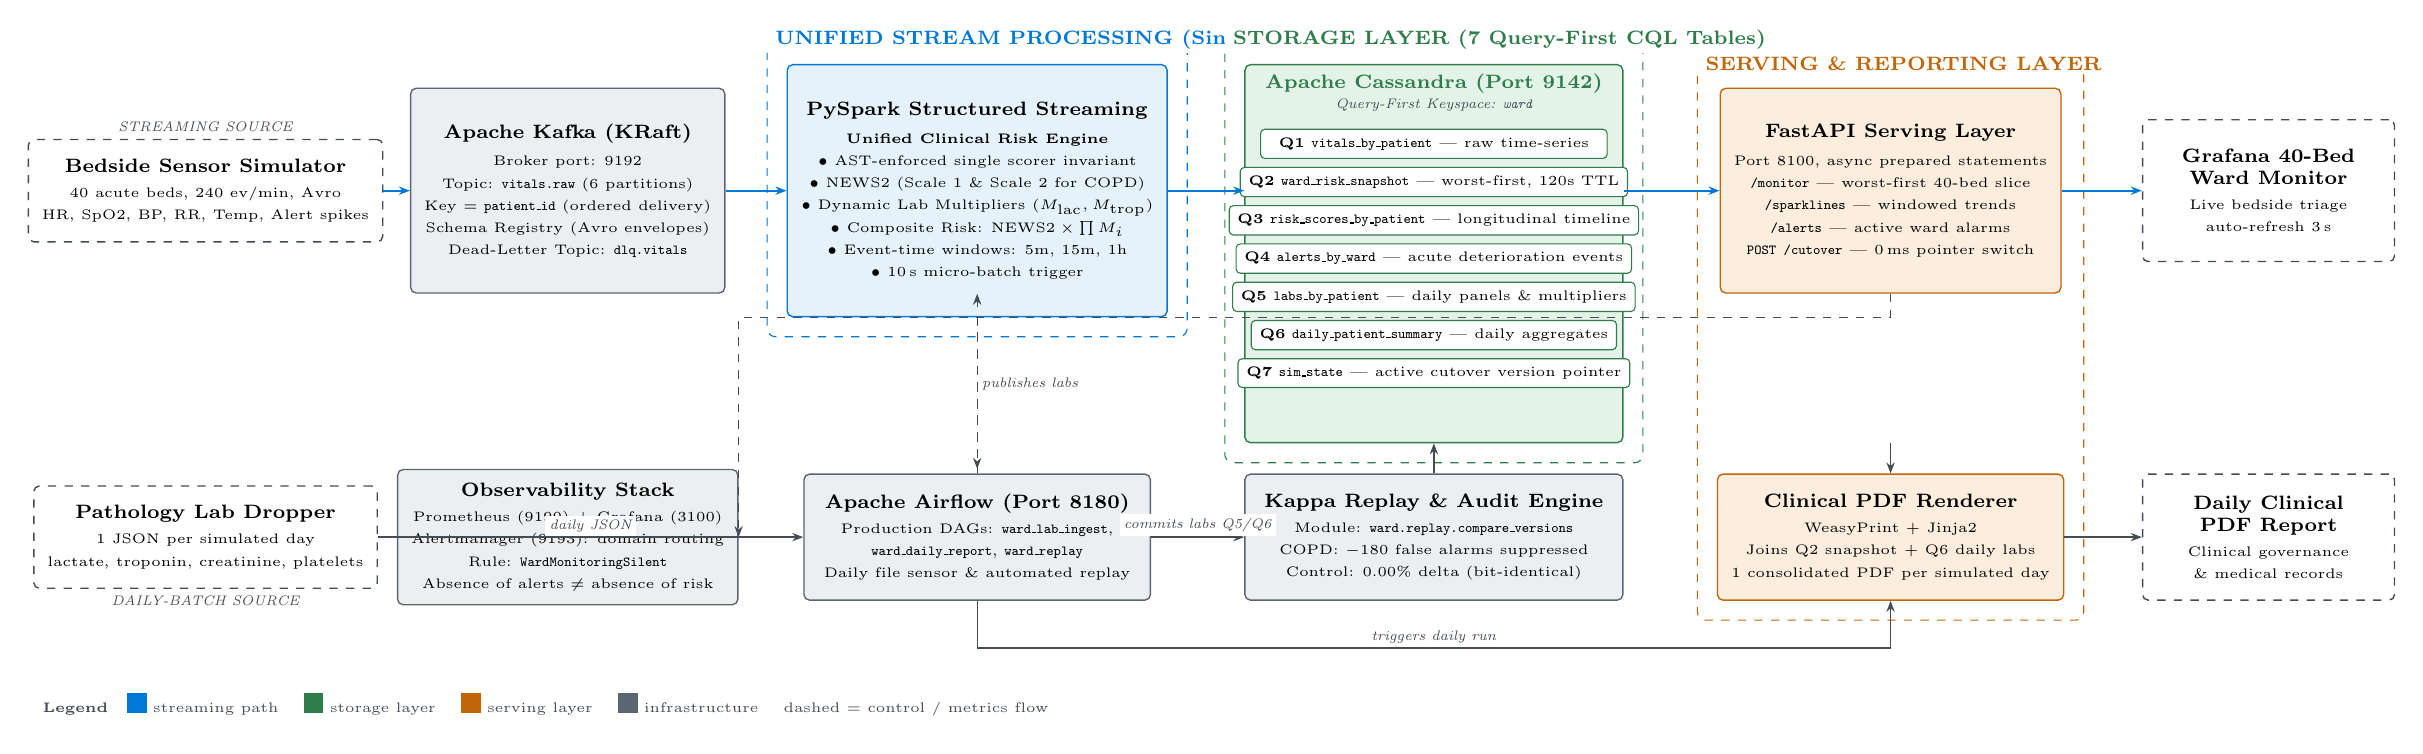
\begin{tikzpicture}[x=10mm, y=10mm]

% ===========================================================================
% 1. SOURCES (Left column, x = 0)
% ===========================================================================
\node[ext, minimum width=34mm, minimum height=13mm] (vitals) at (0, 2.2)
  {\textbf{Bedside Sensor Simulator}\\[1pt]\tiny 40 acute beds, 240 ev/min, Avro\\\tiny HR, SpO2, BP, RR, Temp, Alert spikes};
\node[lbl, above=1pt of vitals.north] {STREAMING SOURCE};

\node[ext, minimum width=34mm, minimum height=13mm] (labs) at (0, -2.2)
  {\textbf{Pathology Lab Dropper}\\[1pt]\tiny 1 JSON per simulated day\\\tiny lactate, troponin, creatinine, platelets};
\node[lbl, below=1pt of labs.south] {DAILY-BATCH SOURCE};

% ===========================================================================
% 2. INGESTION LAYER (x = 4.6)
% ===========================================================================
\node[infra, minimum width=38mm, minimum height=26mm] (kafka) at (4.6, 2.2)
  {\textbf{Apache Kafka (KRaft)}\\[2pt]\tiny Broker port: 9192\\\tiny Topic: \texttt{vitals.raw} (6 partitions)\\\tiny Key = \texttt{patient\_id} (ordered delivery)\\\tiny Schema Registry (Avro envelopes)\\\tiny Dead-Letter Topic: \texttt{dlq.vitals}};

\node[infra, minimum width=38mm, minimum height=16mm] (obs) at (4.6, -2.2)
  {\textbf{Observability Stack}\\[1pt]\tiny Prometheus (9190) + Grafana (3100)\\\tiny Alertmanager (9193): domain routing\\\tiny Rule: \texttt{WardMonitoringSilent}\\\tiny Absence of alerts $\ne$ absence of risk};

% ===========================================================================
% 3. STREAM PROCESSING ENGINE (x = 9.8)
% ===========================================================================
\node[stream, minimum width=44mm, minimum height=32mm] (spark) at (9.8, 2.2)
  {\textbf{PySpark Structured Streaming}\\[2pt]\tiny\textbf{Unified Clinical Risk Engine}\\\tiny $\bullet$ AST-enforced single scorer invariant\\\tiny $\bullet$ NEWS2 (Scale 1 \& Scale 2 for COPD)\\\tiny $\bullet$ Dynamic Lab Multipliers ($M_{\text{lac}}, M_{\text{trop}}$)\\\tiny $\bullet$ Composite Risk: $\text{NEWS2} \times \prod M_i$\\\tiny $\bullet$ Event-time windows: 5m, 15m, 1h\\\tiny $\bullet$ 10\,s micro-batch trigger};

\node[infra, minimum width=44mm, minimum height=16mm] (airflow) at (9.8, -2.2)
  {\textbf{Apache Airflow (Port 8180)}\\[1pt]\tiny Production DAGs: \texttt{ward\_lab\_ingest},\\\tiny \texttt{ward\_daily\_report}, \texttt{ward\_replay}\\\tiny Daily file sensor \& automated replay};

% ===========================================================================
% 4. STORAGE LAYER (x = 15.6)
% ===========================================================================
\node[store, minimum width=48mm, minimum height=48mm] (cass) at (15.6, 1.4) {};
\node[font=\scriptsize\bfseries, text=storegreen, anchor=north] at (cass.north)
  {Apache Cassandra (Port 9142)};
\node[font=\tiny\itshape, text=edgegrey, below=3.2mm of cass.north] (cql_title)
  {Query-First Keyspace: \texttt{ward}};

\node[cqlbox, below=1mm of cql_title, minimum width=44mm] (q1)
  {\textbf{Q1} \texttt{vitals\_by\_patient} \textemdash\ raw time-series};
\node[cqlbox, below=1mm of q1, minimum width=44mm] (q2)
  {\textbf{Q2} \texttt{ward\_risk\_snapshot} \textemdash\ worst-first, 120s TTL};
\node[cqlbox, below=1mm of q2, minimum width=44mm] (q3)
  {\textbf{Q3} \texttt{risk\_scores\_by\_patient} \textemdash\ longitudinal timeline};
\node[cqlbox, below=1mm of q3, minimum width=44mm] (q4)
  {\textbf{Q4} \texttt{alerts\_by\_ward} \textemdash\ acute deterioration events};
\node[cqlbox, below=1mm of q4, minimum width=44mm] (q5)
  {\textbf{Q5} \texttt{labs\_by\_patient} \textemdash\ daily panels \& multipliers};
\node[cqlbox, below=1mm of q5, minimum width=44mm] (q6)
  {\textbf{Q6} \texttt{daily\_patient\_summary} \textemdash\ daily aggregates};
\node[cqlbox, below=1mm of q6, minimum width=44mm] (q7)
  {\textbf{Q7} \texttt{sim\_state} \textemdash\ active cutover version pointer};

\node[infra, minimum width=48mm, minimum height=16mm] (replay) at (15.6, -2.2)
  {\textbf{Kappa Replay \& Audit Engine}\\[1pt]\tiny Module: \texttt{ward.replay.compare\_versions}\\\tiny COPD: $-180$ false alarms suppressed\\\tiny Control: 0.00\% delta (bit-identical)};

% ===========================================================================
% 5. SERVING & REPORTING LAYER (x = 21.4)
% ===========================================================================
\node[serv, minimum width=38mm, minimum height=26mm] (api) at (21.4, 2.2)
  {\textbf{FastAPI Serving Layer}\\[2pt]\tiny Port 8100, async prepared statements\\\tiny \texttt{/monitor} \textemdash\ worst-first 40-bed slice\\\tiny \texttt{/sparklines} \textemdash\ windowed trends\\\tiny \texttt{/alerts} \textemdash\ active ward alarms\\\tiny \texttt{POST /cutover} \textemdash\ 0\,ms pointer switch};

\node[serv, minimum width=38mm, minimum height=16mm] (report_renderer) at (21.4, -2.2)
  {\textbf{Clinical PDF Renderer}\\[1pt]\tiny WeasyPrint + Jinja2\\\tiny Joins Q2 snapshot + Q6 daily labs\\\tiny 1 consolidated PDF per simulated day};

% ===========================================================================
% 6. CONSUMERS & VIEWS (x = 26.2)
% ===========================================================================
\node[ext, minimum width=32mm, minimum height=18mm] (dash) at (26.2, 2.2)
  {\textbf{Grafana 40-Bed}\\\textbf{Ward Monitor}\\[1pt]\tiny Live bedside triage\\\tiny auto-refresh 3\,s};

\node[ext, minimum width=32mm, minimum height=16mm] (pdf_out) at (26.2, -2.2)
  {\textbf{Daily Clinical}\\\textbf{PDF Report}\\[1pt]\tiny Clinical governance\\\tiny \& medical records};

% ===========================================================================
% EDGES & CONNECTIONS
% ===========================================================================
% Streaming path
\draw[streamflow] (vitals.east) -- (kafka.west);
\draw[streamflow] (kafka.east) -- (spark.west);
\draw[streamflow] (spark.east) -- (cass.west |- spark.east);
\draw[streamflow] (cass.east |- api.west) -- (api.west);
\draw[streamflow] (api.east) -- (dash.west);

% Daily batch labs path
\draw[flow] (labs.east) -- node[lbl, above] {daily JSON} (airflow.west);
\draw[flow, dashed] (airflow.north) -- node[lbl, right] {publishes labs} (kafka.south -| airflow.north);
\draw[flow] (airflow.east) -- node[lbl, above] {commits labs Q5/Q6} (replay.west);
\draw[flow] (replay.north) -- (cass.south);

% Reporting path
\draw[flow] (airflow.south) -- ++(0,-0.6) -| node[lbl, pos=0.25, above] {triggers daily run} (report_renderer.south);
\draw[flow] (cass.south -| report_renderer.north) -- (report_renderer.north);
\draw[flow] (report_renderer.east) -- (pdf_out.west);

% Observability telemetry
\draw[flow, dashed] (spark.south) -- (obs.north -| spark.south);
\draw[flow, dashed] (api.south) -- ++(0,-0.3) -| (obs.east);

% ===========================================================================
% BACKGROUND ZONES & TITLES
% ===========================================================================
\begin{scope}[on background layer]
  \node[zone, fit=(spark), draw=streamblue] (zstream) {};
  \node[zone, fit=(cass), draw=storegreen] (zstore) {};
  \node[zone, fit=(api)(report_renderer), draw=servorange] (zserv) {};
\end{scope}

\node[ztitle, text=streamblue, above=0.5mm of zstream.north west, anchor=west]
  {UNIFIED STREAM PROCESSING (Single Scorer Invariant)};
\node[ztitle, text=storegreen, above=0.5mm of zstore.north west, anchor=west]
  {STORAGE LAYER (7 Query-First CQL Tables)};
\node[ztitle, text=servorange, above=0.5mm of zserv.north west, anchor=west]
  {SERVING \& REPORTING LAYER};

% ===========================================================================
% LEGEND
% ===========================================================================
\node[font=\tiny, align=left, below=12mm of labs.south west, anchor=north west, text=edgegrey]
  {\textbf{Legend}\quad
   \textcolor{streamblue}{\rule{2.5mm}{2.5mm}}~streaming path \quad
   \textcolor{storegreen}{\rule{2.5mm}{2.5mm}}~storage layer \quad
   \textcolor{servorange}{\rule{2.5mm}{2.5mm}}~serving layer \quad
   \textcolor{infragrey}{\rule{2.5mm}{2.5mm}}~infrastructure \quad
   dashed~=~control / metrics flow};

\end{tikzpicture}
\end{document}
